\documentclass[main.tex]{subfiles}
 
\begin{document}

\part{Investigating slow slip using wavelets}

\chapter{Introduction}

\begin{itemize}
	\item Some generalities about slow slip and tremor
	\item A few words about what wavelets are
	\item Short bibliography about what has been done (master Sequoia Alba + papers by Ohtani and Wei)
\end{itemize}

The goal of this research work is to study the change over time in the spectral content of recordings of surface displacement by GPS stations, in order to detect slow slip events.

What I hope to do with that:

\begin{itemize}

\item Maybe by combining wavelet analyses of several channels and several stations, we will be able to detect smaller inter-ETS events, which can currently be observed in the tremor catalogs, but not in the GPS data.

\item Maybe by looking at the wavelet details at larger scale, we could see some long term events (but we need to find a way to deal with the missing data before that).

\item We could use wavelets to do some denoising of the vertical component of the GPS data. That could be useful to invert the slip at the surface and get the maximum depth of the slip on the plate boundary.

\item Which region would be more interesting to study? All Cascadia? Only some areas not very well covered?

\end{itemize} 

\section{New Zealand}

Slow slip in 2004 but no tremor. Instead, increase in microseismicity (Delahaye et al., 2009). Possible explanation is shallower depth (15-20 km) of the slow slip.

Shallow (15-20 km) and deep (25-60 km) slow slip events. Tremor downdip of the slow slip (Bartlow et al., 2014) but microseismicity.

Challenging tremor detection. Most abundant during large magnitude SSE. Deep inland tremor with possible undetected long-term SSE. (Todd and Schwartz, 2016)

\chapter{Data}

We use the GPS data collected and made available on the website of the Pacific Northwest Geodetic Array (\href{http://www.geodesy.cwu.edu/}{PANGA}), from Central Washington University. Three types of time series are available:

\begin{itemize}
\item Raw data recorded by the GPS stations, after GIPSY postprocessing.
\item Detrended data, for which a linear trend corresponding to the secular plate motion has been removed from the data.
\item Cleaned data, for which the linear trend, steps due to earthquakes or hardware upgrades, and annual and semi-annual sinusoids signals have been simultaneously estimated and removed following Szeliga \textit{et al.} (2008 ~\cite{SZE_2008}). Surface loading due to hydrology and atmospheric pressure introduces an annual signal in the GPS time series with respect to a global reference frame. This annually repeating component also introduces power at all harmonic frequencies, thus it may also be necessary to remove a semi-annual sinusoid from the raw data (Blewitt and Lavall\'ee, 2002 ~\cite{BLE_2002}).
\end{itemize}

For each GPS station, the website provides a file for the three components of the displacement (latitude, longitude, and vertical), and each file contains three columns, corresponding to the time, the displacement (in millimetres), and the error. The data are recorded once a day. \\

The raw data are filtered with the function $f (t)$ to obtain the detrended, and then the cleaned data:

\begin{equation}
f (t) = \textrm{line} (t) + \textrm{(annual + semi-annual)} (t) + \textrm{jumps} (t)
\end{equation}

with:

\begin{equation}
\textrm{line} (t) = p_1 + p_2 t
\end{equation}

\begin{equation}
\textrm{(annual + semi-annual)} (t) = p_3 \sin (2 \pi t + p_4) + p_5 \sin (4 \pi t + p_6)
\end{equation}

\begin{equation}
\textrm{jumps} (t) = \sum_{i = 1}^{n} p_i \textrm{Heaviside} (t - t_i)
\end{equation}

The values of the $p_i$ and $t_i$ are given at the beginning of each file. The best linear unbiased estimates of the model parameters $p_i$ are computed using an orthogonal-triangular decomposition, or QR-factorization (Nikolaidis, 2002 ~\cite{NIK_2002}).

\chapter{Method}

The Discrete Wavelet Transform (DWT) is an orthonormal transform that uses a sequence of filtering operations to associate a time series $X_t (t = 0 , ... , N - 1)$ written in the traditional orthonormal basis:

\begin{equation}
\bm{X} = X_0 \begin{pmatrix} 1 \\ 0 \\ 0 \\ . \\ . \\ . \\ 0 \end{pmatrix}
+ X_1 \begin{pmatrix} 0 \\ 1 \\ 0 \\ . \\ . \\ . \\ 0 \end{pmatrix}
+ X_2 \begin{pmatrix} 0 \\ 0 \\ 1 \\ . \\ . \\ . \\ 0 \end{pmatrix}
+ ... + X_{N - 1} \begin{pmatrix} 0 \\ 0 \\ 0 \\ . \\ . \\ . \\ 1 \end{pmatrix}
\end{equation}

with the wavelet coefficients $W_t (t = 0 , ... , N - 1)$, which is the same time series written in another orthonormal basis:

\begin{equation}
\bm{X} = W_0 \begin{pmatrix} \mathcal{W}_{0 , 0} \\ \mathcal{W}_{0 , 1} \\ \mathcal{W}_{0 , 2} \\ . \\ . \\ . \\ \mathcal{W}_{0 , N - 1} \end{pmatrix}
+ W_1 \begin{pmatrix} \mathcal{W}_{1 , 0} \\ \mathcal{W}_{1 , 1} \\ \mathcal{W}_{1 , 2} \\ . \\ . \\ . \\ \mathcal{W}_{1 , N - 1} \end{pmatrix}
+ W_2 \begin{pmatrix} \mathcal{W}_{2 , 0} \\ \mathcal{W}_{2 , 1} \\ \mathcal{W}_{2 , 2} \\ . \\ . \\ . \\ \mathcal{W}_{2 , N - 1} \end{pmatrix}
+ ... + W_{N - 1} \begin{pmatrix} \mathcal{W}_{N - 1 , 0} \\ \mathcal{W}_{N - 1 , 1} \\ \mathcal{W}_{N - 1 , 2} \\ . \\ . \\ . \\ \mathcal{W}_{N - 1 , N - 1} \end{pmatrix}
\end{equation}

where the $\bm{\mathcal{W}_{t , .}} \left( t = 0 , ... , N - 1 \right)$ are the wavelet basis vectors. The main advantage of the wavelet transform is that it captures information about both the frequency and the temporal content of the input data. This is contrasted with the Fourier transform, which characterizes the amplitude and phase of the frequency content only. Indeed, a local perturbation of the initial time series will affect all the coefficients of the Fourier transform, whereas it will only affect a few wavelet coefficients around the time of the perturbation. \\ 

The first $\frac{N}{2}$ $\bm{\mathcal{W}_{t , .}} \left( t = 0 , ... , \frac{N}{2} - 1 \right)$ wavelet basis vectors are circularly shifted with each other:

\begin{equation}
\mathcal{W}_{k , j} = \mathcal{W}_{i , j + 2 \left( i - k \right)}
\end{equation}

and their Fourier transform has a nominal frequency band of $\lbrack \frac{1}{4 dt} ; \frac{1}{2 dt} \rbrack$, where $dt$ is the time step of the time series. We can write their coordinates as:

\begin{equation}
\mathcal{W}_{t , l} = h_{2 t + 1 - l \mod N}^o \text{, } t = 0 , ... , \frac{N}{2} - 1 \text{, } l = 0 , ... , N - 1
\end{equation}

where $h_l^o \left( l = 0 , ... , N - 1 \right)$ is the wavelet filter. \\

The first wavelet vector $\bm{W_1}$ has length $\frac{N}{2}$, and is associated with changes on scale $\tau_1 = dt$. We can get its coefficients $W_{1 , t} \left(t = 0 , ... , \frac{N}{2} - 1 \right)$ by computing the scalar product of the first $\frac{N}{2}$ $\bm{\mathcal{W}_{t , .}} \left( t = 0 , ... , \frac{N}{2} - 1 \right)$ wavelet basis vectors with the time series $\bm{X}$:

\begin{equation}
W_{1 , t} = \sum_{j = 0}^{N - 1} \mathcal{W}_{t , j} X_j \text{, } t = 0 , ... , \frac{N}{2} - 1
\end{equation}

The new time series $\bm{W_1}$ has time step $2 dt$, and corresponds to the filtering of the original time series with a filter with nominal frequency interval $\lbrack \frac{1}{4 dt} ; \frac{1}{2 dt} \rbrack$. \\

The next $\frac{N}{4}$ $\bm{\mathcal{W}_{t , .}} \left( t = \frac{N}{2} , .... , \frac{3 N}{4} - 1 \right)$ wavelet basis vectors are also circularly shifted with each other:

\begin{equation}
\mathcal{W}_{k , j} = \mathcal{W}_{i , j + 4 \left( i - k \right)}
\end{equation}

and their Fourier transform has a nominal frequency band of $\lbrack \frac{1}{8 dt} ; \frac{1}{4 dt} \rbrack$. We can write their coordinates as:

\begin{equation}
\mathcal{W}_{\frac{N}{2} + t , l} = \sum_{j = 0}^{N - 1} g_{j - l \mod N}^o h_{4 t + 3 - j \mod N}^{o \uparrow} \text{, } t = 0 , ... , \frac{N}{4} - 1 \text{, } l = 0 , ... , N - 1
\end{equation}

where $\bm{h^{o \uparrow}}$ is formed by inserting a $0$ between each of the elements of $\bm{h^o}$, and $g_l^o \left( l = 0 , ... , N - 1 \right)$ is the scaling filter defined by:

\begin{equation}
g_l^o = \left( - 1 \right) ^{l + 1} h_{N - 1 - l}^o \text{, } l = 0 , ... , N - 1
\end{equation}

The second wavelet vector $\bm{W_2}$ has length $\frac{N}{4}$, and is associated with changes on scale $\tau_2 = 2 dt$. We can get its coefficients $W_{2 , t} \left( t = 0 , ... , \frac{N}{4} - 1 \right)$ by computing the scalar product of the next $\frac{N}{4}$ $\bm{\mathcal{W}_{t , .}} \left( t = \frac{N}{2} , ... , \frac{3 N}{4} - 1 \right)$ wavelet basis vectors with the time series $\bm{X}$:

\begin{equation}
W_{2 , t} = \sum_{j = 0}^{N - 1} \mathcal{W}_{\frac{N}{2} + t , j} X_j \text{, } t = 0 , ... , \frac{N}{4} - 1
\end{equation}

The new time series $\bm{W_2}$ has time step $4 dt$, and corresponds to the filtering of the original time series with a filter with nominal frequency interval $\lbrack \frac{1}{8 dt} ; \frac{1}{4 dt} \rbrack$. \\

At the level $J$, we can write the orthonormal transform as:

\begin{equation}
\bm{W} = \mathcal{W} \bm{X} \text{ or } \begin{pmatrix} \bm{W_1} \\ \bm{W_2} \\ \bm{W_3} \\ . \\ . \\ . \\ \bm{W_J} \\ \bm{V_J} \end{pmatrix}
= \begin{pmatrix} \mathcal{W}_1 \bm{X} \\ \mathcal{W}_2 \bm{X} \\ \mathcal{W}_3 \bm{X} \\ . \\ . \\ . \\ \mathcal{W}_J \bm{X} \\ \mathcal{V}_J \bm{X} \end{pmatrix}
\end{equation}

Each of the wavelet vectors $\bm{W_j} \left( j = 1 , ... , J \right)$ has length $\frac{N}{2^j}$, has a time step of $2^j dt$, and corresponds to the filtering of the initial time series by a filter of nominal frequency band $\lbrack \frac{1}{dt 2^{j + 1}} ; \frac{1}{dt 2^j} \rbrack$. The scaling vector $\bm{V_J}$ has length $\frac{N}{2^J}$, has a time step of $2^J dt$, and corresponds to the filtering of the initial time series by a filter of nominal frequency band $\lbrack 0 ; \frac{1}{dt 2^{J + 1}} \rbrack$. \\

We can compute iteratively the wavelet vectors and the scaling vector using a pyramid algorithm and the wavelet filter $h_l^o \left( l = 0 , ... , N - 1 \right)$ and the scaling filter $g_l^o \left( l = 0 , ... , N - 1 \right)$:

\begin{equation}
W_{j , t} = \sum_{l = 0}^{N - 1} h_l^o V_{j - 1 , 2 t + 1 - l \mod N_{j - 1}} \text{ and } V_{j , t} = \sum_{l = 0}^{N - 1} g_l^o V_{j - 1 , 2 t + 1 - l \mod N_{j - 1}} \text{, } t = 0 , ... , N_j - 1
\end{equation}

where $N_j = \frac{N}{2^j}$ and $\bm{V_0} = \bm{X}$. \\

We can then compute the $j$th level detail $\bm{D_j} \left( j = 1 , ... , J \right)$, which is a vector of length $N$, defined by $\bm{D_j} = \mathcal{W}_j^T \bm{W_j}$ and the $J$th level smooth $\bm{S_J}$, which is a vector of length $N$, defined by $\bm{S_J} = \mathcal{V}_J^T \bm{V_J}$, and we get the multiresolution analysis (MRA) of $\bm{X}$:

\begin{equation}
\bm{X} = \sum_{j = 1}^{J} \bm{D_j} + \bm{S_J}
\end{equation}

One main advantage of the DWT is that it is an orthonormal transform, and thus we can write the analysis of variance (ANOVA):

\begin{equation}
\left\Vert \bm{X} \right\Vert ^2 = \left\Vert \bm{W} \right\Vert ^2 = \sum_{j = 1}^{J} \left\Vert \bm{W_j} \right\Vert ^2 + \left\Vert \bm{V_J} \right\Vert ^2 = \sum_{j = 1}^{J} \left\Vert \bm{D_j} \right\Vert ^2 + \left\Vert \bm{S_J} \right\Vert ^2
\end{equation}

Moreover, the DWT can be computed using $O \left( N \right)$ multiplications. \\

However, the DWT present several disadvantages:

\begin{itemize}
	\item The length of the time series must be a multiple of $2^J$ where $J$ is the level of the DWT decomposition.
	\item The time step of the wavelet vector $\bm{W_j}$ is $2^j dt$, which may not correspond to the time when some interesting phenomenon is visible on the original time series.
	\item When we circularly shift the time series, the corresponding wavelet coefficients, details and smooths are not a circularly shifted version of the wavelet coefficients, details and smooths of the original time series. Thus, the values of the wavelet coefficients, details and smooths are strongly dependent on the time when we start experimentally gathering the data.
	\item When we filter the time series to obtain the details and smooths, we introduce a phase shift, which makes difficult to line up meaningfully the features of the MRA with the original time series.
\end{itemize}

To get rid of these problems, we introduce the Maximum Overlap Discrete Wavelet Transform (MODWT). The MODWT transforms the time series $X_t \left( t = 0, ... , N - 1 \right)$ into J wavelet vectors $\bm{\widetilde{W}_j} \left( j = 1 , ... , J \right)$ of length $N$ and a scaling vector $\bm{\widetilde{V}_J}$ of length $N$. Each wavelet vector $\bm{\widetilde{W}_j}$ corresponds to the filtering of the original time series with a filter with nominal frequency band $\lbrack \frac{1}{dt 2^{j + 1}} ; \frac{1}{dt 2^j} \rbrack$. The scaling vector $\bm{\widetilde{V}_J}$ corresponds to the filtering of the original time series with a filter with nominal frequency band $\lbrack 0 ; \frac{1}{dt 2^{j + 1}} \rbrack$. \\

We can write the transformation as:

\begin{equation}
\bm{\widetilde{W}_j} = \widetilde{\mathcal{W}_j} \bm{X} \text{ and } \bm{\widetilde{V}_J} = \widetilde{\mathcal{V}_J} \bm{X}
\end{equation}

$ \widetilde{\mathcal{W}}_j$ and $\widetilde{\mathcal{V}}_J$ are related to $\mathcal{W}_j$ and $\mathcal{V}_J$ by:

\begin{equation}
\widetilde{\mathcal{W}}_{j, t l} = \widetilde{h}_{j , t - l \mod N}^o \text{, } \mathcal{W}_{j, t l} = h_{j , 2^j \left( t + 1 \right) - 1 - l \mod N}^o \text{ and } \widetilde{h}_{j , l}^o = \frac{h_{j , l}^o}{2^{j/2}}
\end{equation}

As is the case for the DWT, we can compute iteratively the MODWT wavelet vectors and the scaling vector using a pyramid algorithm and the wavelet filter $\widetilde{h}_l^o \left( l = 0 , ... , N - 1 \right)$ and the scaling filter $\widetilde{g}_l^o \left( l = 0 , ... , N - 1 \right)$:

\begin{equation}
\widetilde{W}_{j , t} = \sum_{l = 0}^{N - 1} \widetilde{h}_l^o V_{j - 1 , t - 2^{j - 1} l \mod N} \text{ and } \widetilde{V}_{j , t} = \sum_{l = 0}^{N - 1} \widetilde{g}_l^o V_{j - 1 , t - 2^{j - 1} l \mod N} \text{, } t = 0 , ... , N - 1
\end{equation}

where $\widetilde{h}_l^o = \frac{h_l^o}{\sqrt{2}} \left( l = 0 , ... , N - 1 \right)$,  $\widetilde{g}_l^o = \frac{g_l^o}{\sqrt{2}} \left( l = 0 , ... , N - 1 \right)$ and $\bm{\widetilde{V}_0} = \bm{X}$. \\

We can then compute the $j$th level detail $\bm{\widetilde{D}_j} \left( j = 1 , ... , J \right)$, which is a vector of length $N$, defined by $\bm{\widetilde{D}_j} = \widetilde{\mathcal{W}}_j^T \bm{\widetilde{W}_j}$ and the $J$th level smooth $\bm{\widetilde{S}_J}$, which is a vector of length $N$, defined by $\bm{\widetilde{S}_J} = \widetilde{\mathcal{V}}_J^T \bm{\widetilde{V}_J}$, and we get the multiresolution analysis (MRA) of $\bm{X}$:

\begin{equation}
\bm{X} = \sum_{j = 1}^{J} \bm{\widetilde{D}_j} + \bm{\widetilde{S}_J}
\end{equation}

and the ANOVA:

\begin{equation}
\left\Vert \bm{X} \right\Vert ^2 = \sum_{j = 1}^{J} \left\Vert \bm{\widetilde{W}_j} \right\Vert ^2 + \left\Vert \bm{\widetilde{V}_J} \right\Vert ^2
\end{equation}

Now, we have the following properties:

\begin{itemize}
	\item The MODWT of a time series can be defined for any length $N$.
	\item The time step of the wavelet vectors $\bm{\widetilde{W}_j}$ and the scaling vector $\bm{\widetilde{V}_J}$ is equal to the time step of the original time series.
	\item When we circularly shift the time series, the corresponding wavelet vectors, scaling vector, details and smooths are shifted by the same amount.
	\item The details and smooths are associated with a zero phase filter, making it easy to line up meaningfully the features of the MRA with the original time series.
\end{itemize}

However, the MODWT has some disadvantages over the DWT:

\begin{itemize}
	\item The MODWT can only be computed using $O \left( N \log_2 N \right)$ multiplications.
	\item We can no longer write the ANOVA for the details and smooths:

\begin{equation}
\left\Vert \bm{X} \right\Vert ^2 \neq \sum_{j = 1}^{J} \left\Vert \bm{\widetilde{D}_j} \right\Vert ^2 + \left\Vert \bm{\widetilde{S}_J} \right\Vert ^2 \text{ and } \left\Vert \bm{\widetilde{W}_j} \right\Vert ^2 \neq \left\Vert \bm{\widetilde{D}_j} \right\Vert ^2
\end{equation}

\end{itemize}

\chapter{Results}

In the following, we show results of the DWT and MODWT analysis of one GPS time series. \\

Computing the DWT or the MODWT of a time series requires computing the convolution product of the time series with the wavelet or the scaling filter. To handle the boundary conditions, we assume that the time series is periodic, and extend accordingly the time series. However, we can only make this assumption when the discontinuity between the beginning and the end of the time series remains small. Therefore, we used the cleaned dataset in order to avoid discontinuities due to the linear trend, and earthquakes or hardware upgrades. In order to analyze the temporal correlation of the slow slip with the tectonic tremor, we also used the tremor catalog of the Pacific Northwest Seismic Network (PNSN, Wech, 2010 ~\cite{WEC_2010}) to get the cumulative number of tremor recorded around the GPS station. The displacement is recorded once a day at every GPS station. However, there are many missing data points. We chose the GPS station PGC5, located in southern Vancouver Island, near Victoria. The slow slip events are clearly visible in the longitudinal component of the displacement (see bottom panel of Figure 20.1). Moreover, there are very few missing data for this station. In the following, we have analyzed eight years of GPS data from 2006 to 2014. There are only five days for which the displacement is missing. We replaced the missing data by the average of the displacement on the day before and the displacement on the day after. \\

We first carried out a partial DWT of the time series. To choose the appropriate wavelet filter, we computed the Normalized Partial Energy Sequence (NPES) of the wavelet coefficients and of the time series for different wavelet filters. It did not seem that there was much difference between the different wavelet filters. In the following, we will compare the wavelet coefficients to the cumulative number of tremor recorded around the GPS station. Therefore, we would like to know with good precision the time shift that should be applied to the wavelet coefficients. Moreover, we would like the length of the wavelet filter to remain small, in order to reduce the number of coefficients that are affected by the interpolation we had to do to replace the missing data. This is why we chose the Daubechies least asymmetric (LA8) wavelet filter in the following analysis. \\

The total duration of a slow slip event is about six weeks. Therefore, we only carried out a partial DWT up to the level 6 (corresponding to a scale of 64 days), because we do not expect to see features at a longer scale in the time series. \\

The wavelet coefficients for level 1 to 6 are shown in Figure 20.1. The red bars correspond to the days where data were missing. The grey bars correspond to the timing of ETS events.  The blue bars correspond to the left and right boundaries outside of which the wavelet coefficients are affected by the boundary conditions. We can clearly see big wavelet coefficients corresponding to the January 2007 ETS event at the levels 5 and 6, to the May 2009 ETS event at the level 5, to the August 2010 ETS event at the level 6, to the September 2012 ETS event at the levels 5 and 6, and to the September 2013 ETS event at the levels 5 and 6.  The May 2008 and August 2011 ETS events are not clearly seen in the wavelet coefficients. \\

\begin{center}
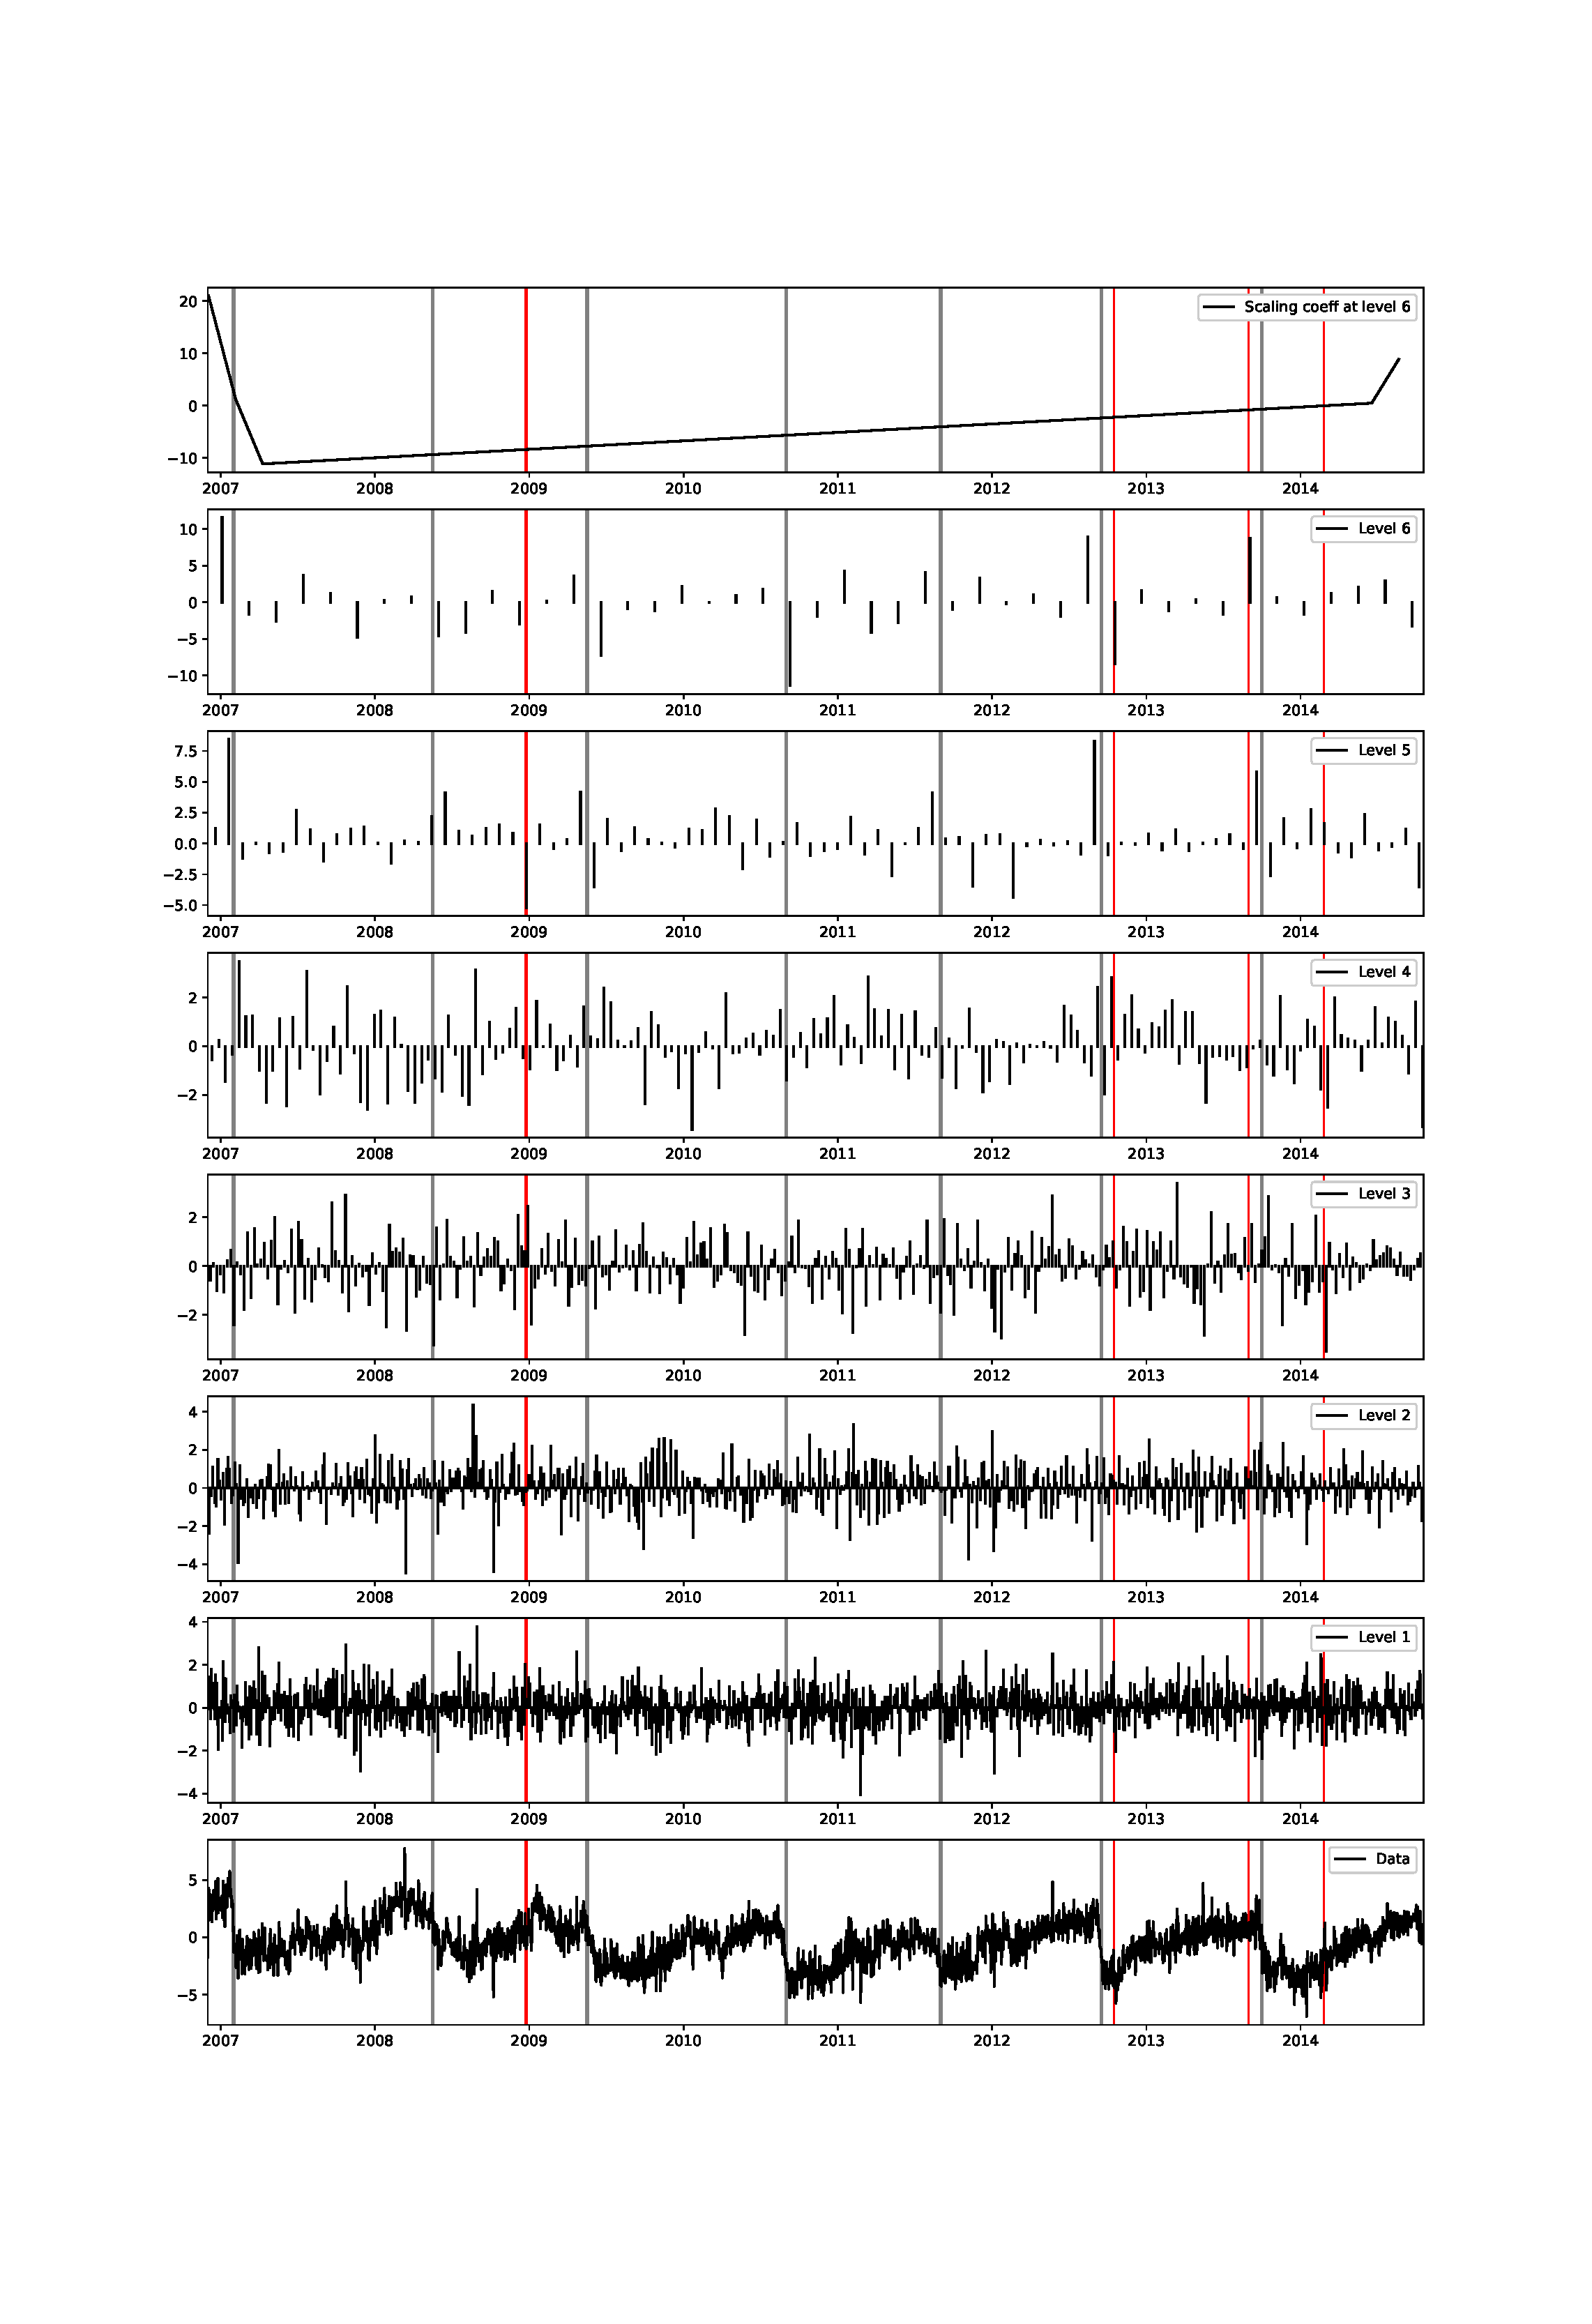
\includegraphics[width=300pt, trim={3.5cm 6cm 3.5cm 6.5cm},clip]{Figures/slowslip_results/Figure_1.eps}
\captionsetup{type=figure}
\captionof{figure}{Partial DWT wavelet coefficients up to level 6 of the longitudinal component of station PGC5. The red bars correspond to the days where data were missing. The grey bars correspond to the timing of ETS events. The blue bars correspond to the left and right boundaries outside of which the wavelet coefficients are affected by the boundary conditions.}
\end{center}

The 5\textsuperscript{th} and 6\textsuperscript{th} level details of the MRA are plotted with the cumulative number of tremor in Figure 20.2. Unfortunately, the tremor catalog from the PNSN website only starts in August 2009. We plotted successively the cumulative number of tremor which source was located less than 20, 40, 60, 80, or 100 kilometres from the GPS station. We can clearly see the August 2010, September 2012 and September 2013 ETS events in the 6\textsuperscript{th} level detail. The August 2011 ETS event is less obvious, but can be seen in the 5\textsuperscript{th} level detail. There is a small increase in the number of tremor in March 2010, but it is not really clear that there is a corresponding peak in the 5\textsuperscript{th} level detail.

\begin{center}
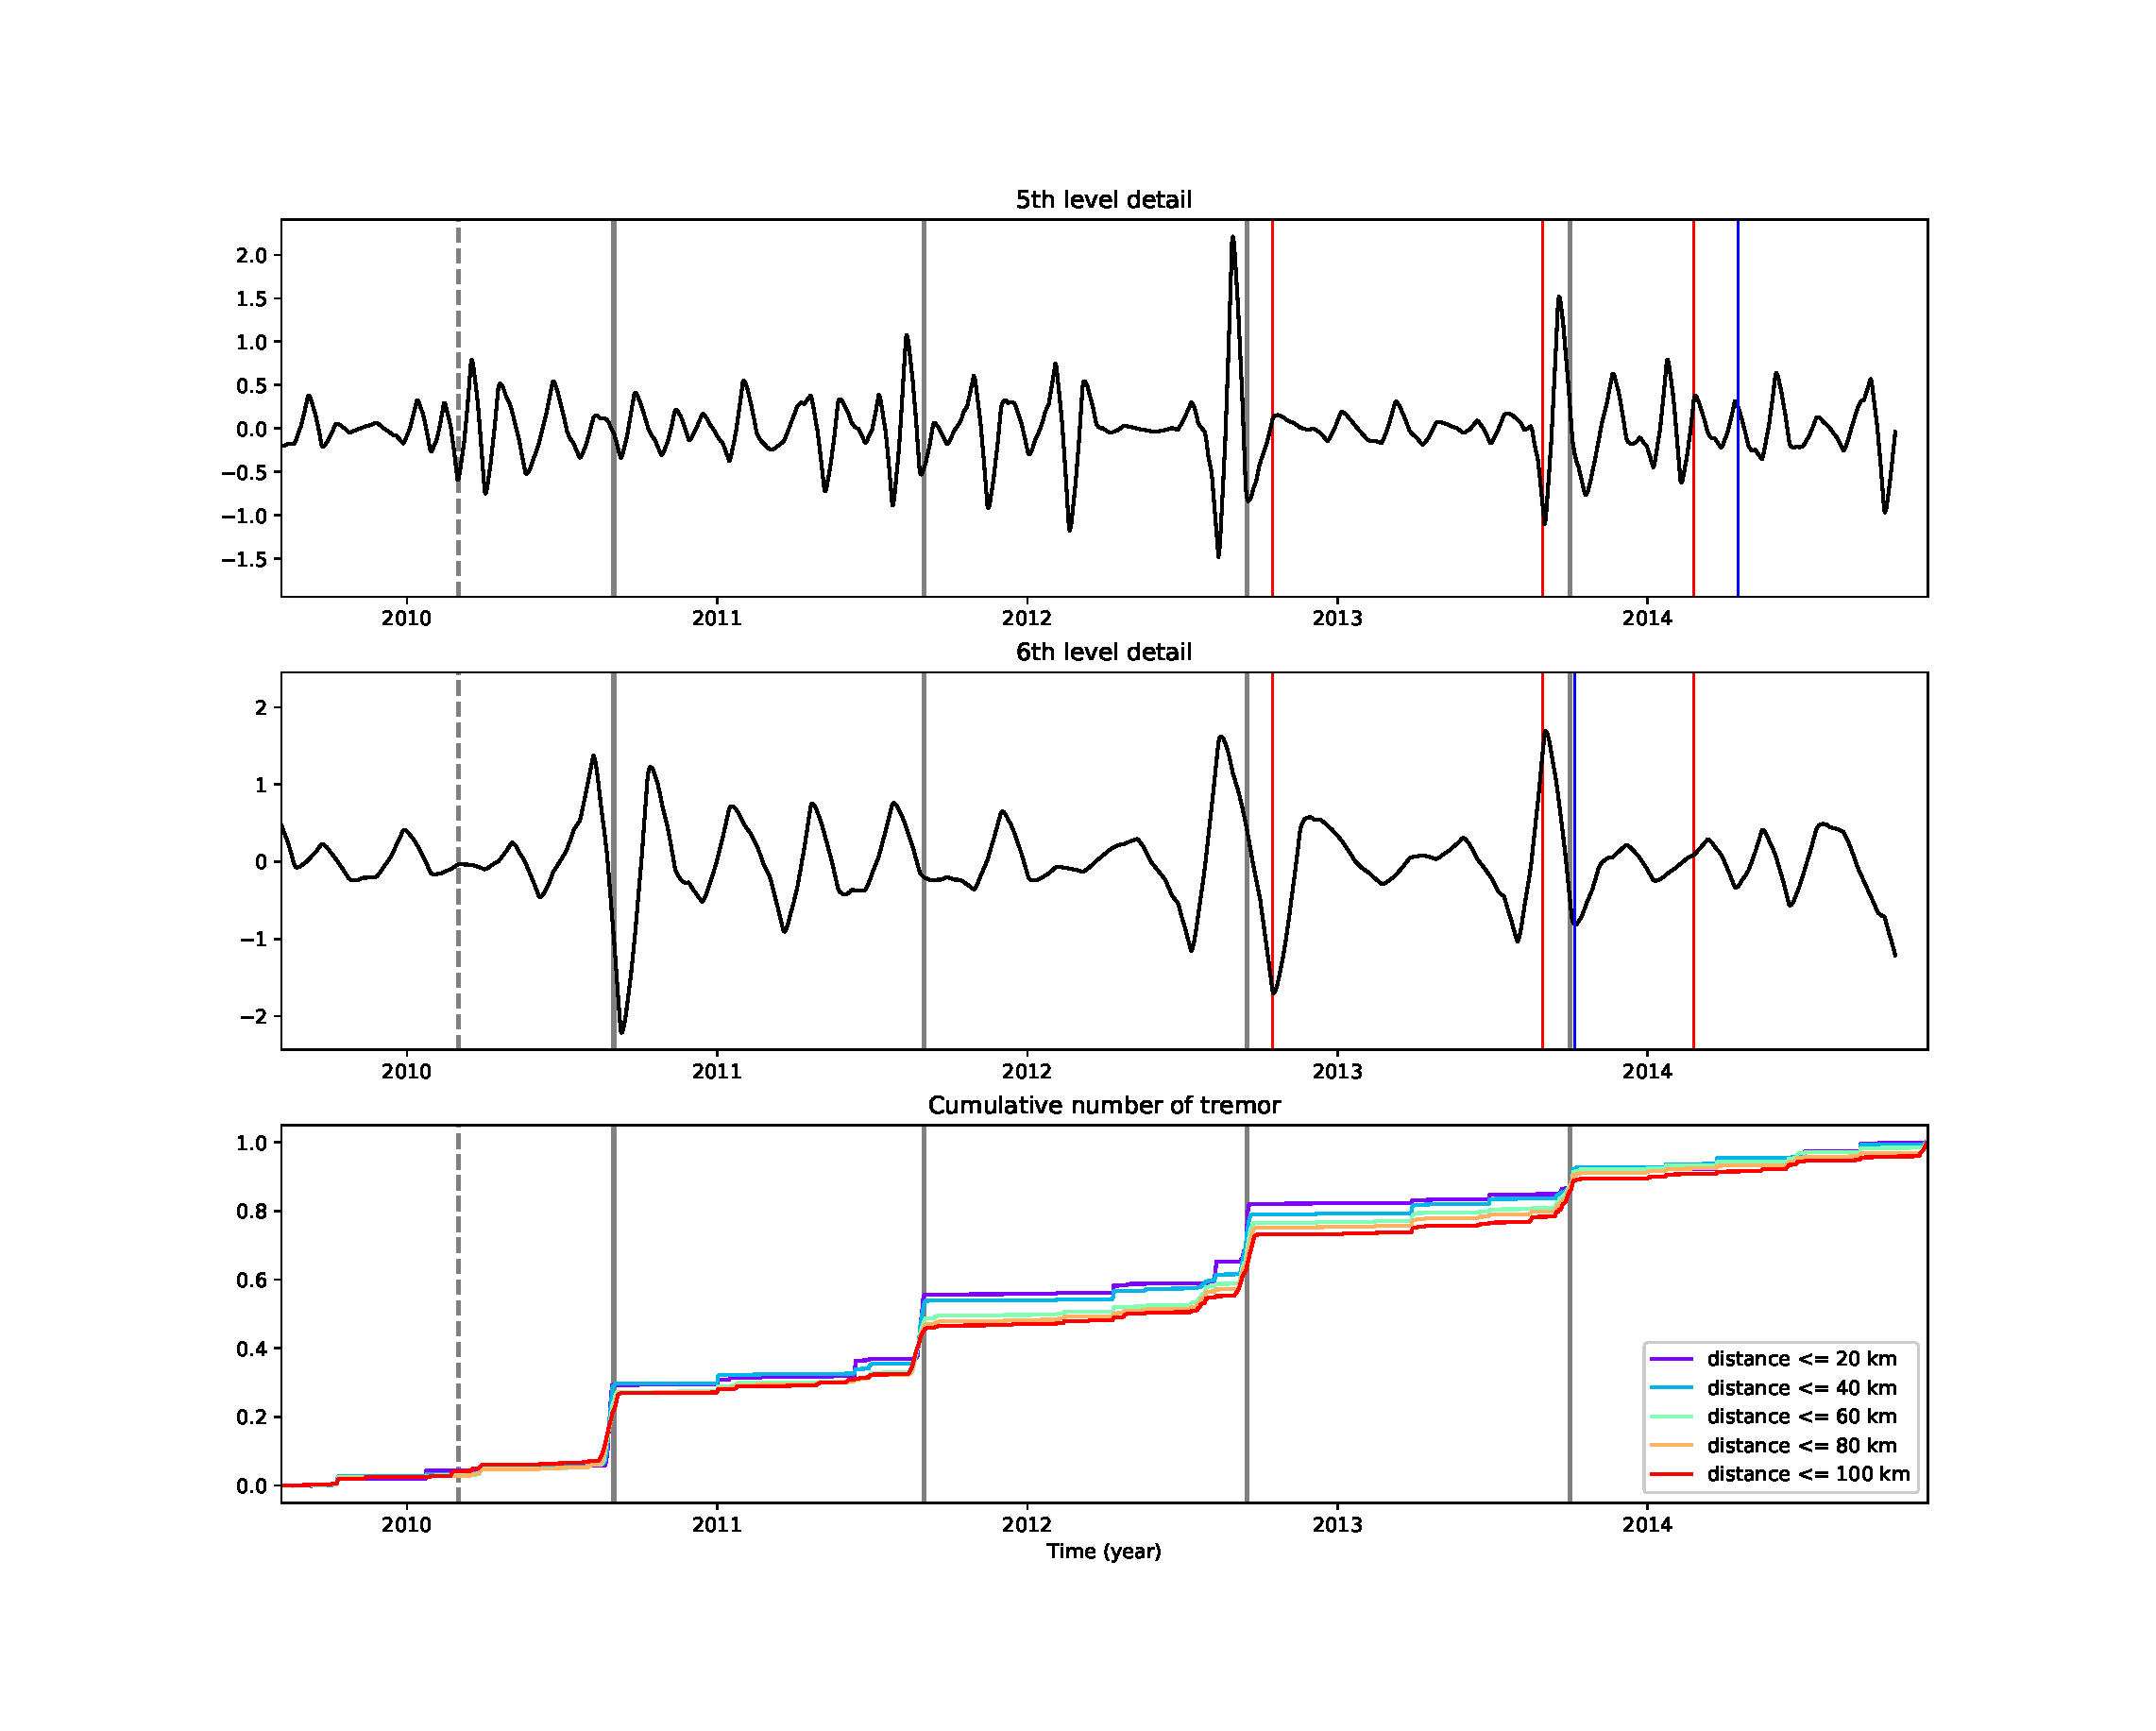
\includegraphics[width=300pt, trim={3.5cm 2.5cm 3.5cm 3cm}, clip]{Figures/slowslip_results/Figure_2.eps}
\captionsetup{type=figure}
\captionof{figure}{5\textsuperscript{th} and 6\textsuperscript{th} level details of the partial DWT analysis of the longitudinal component of station PGC5 (top and middle panel), and cumulative number of tremor
recorded around the GPS station (bottom panel). The red bars correspond to the days where data were missing. The grey bars correspond to the timing of ETS events. The blue bar corresponds to the right boundary outside of which the wavelet coefficients are affected by the boundary conditions.}
\end{center}

The details of the MRA with the partial DWT have a somewhat 'shark fin' look, which is not entirely pleasing. Moreover, the number of days between two ETS events may not correspond to a multiple of a power of 2. Therefore, it would be easier to interpret the wavelet coefficients at each level if their dimensions was the same as the dimension of the original time series. Finally, it would be easier to associate the details and smooths of the MRA with the cumulative number of tremor recorded if they were associated with zero phase filters. Therefore, in the following, we carried out a MODWT analysis on the same time series. \\

The wavelet coefficients for level 1 to 6 are shown in Figure 20.3. We can clearly see peaks corresponding to the January 2007, May 2009, August 2010, September 2012, and September 2013 ETS events in both the level 5 and level 6 coefficients. A peak corresponding to the May 2008 ETS event can be seen in the level 5 coefficients. However, it is still difficult to observe the August 2011 ETS event in the wavelet coefficients. \\

\begin{center}
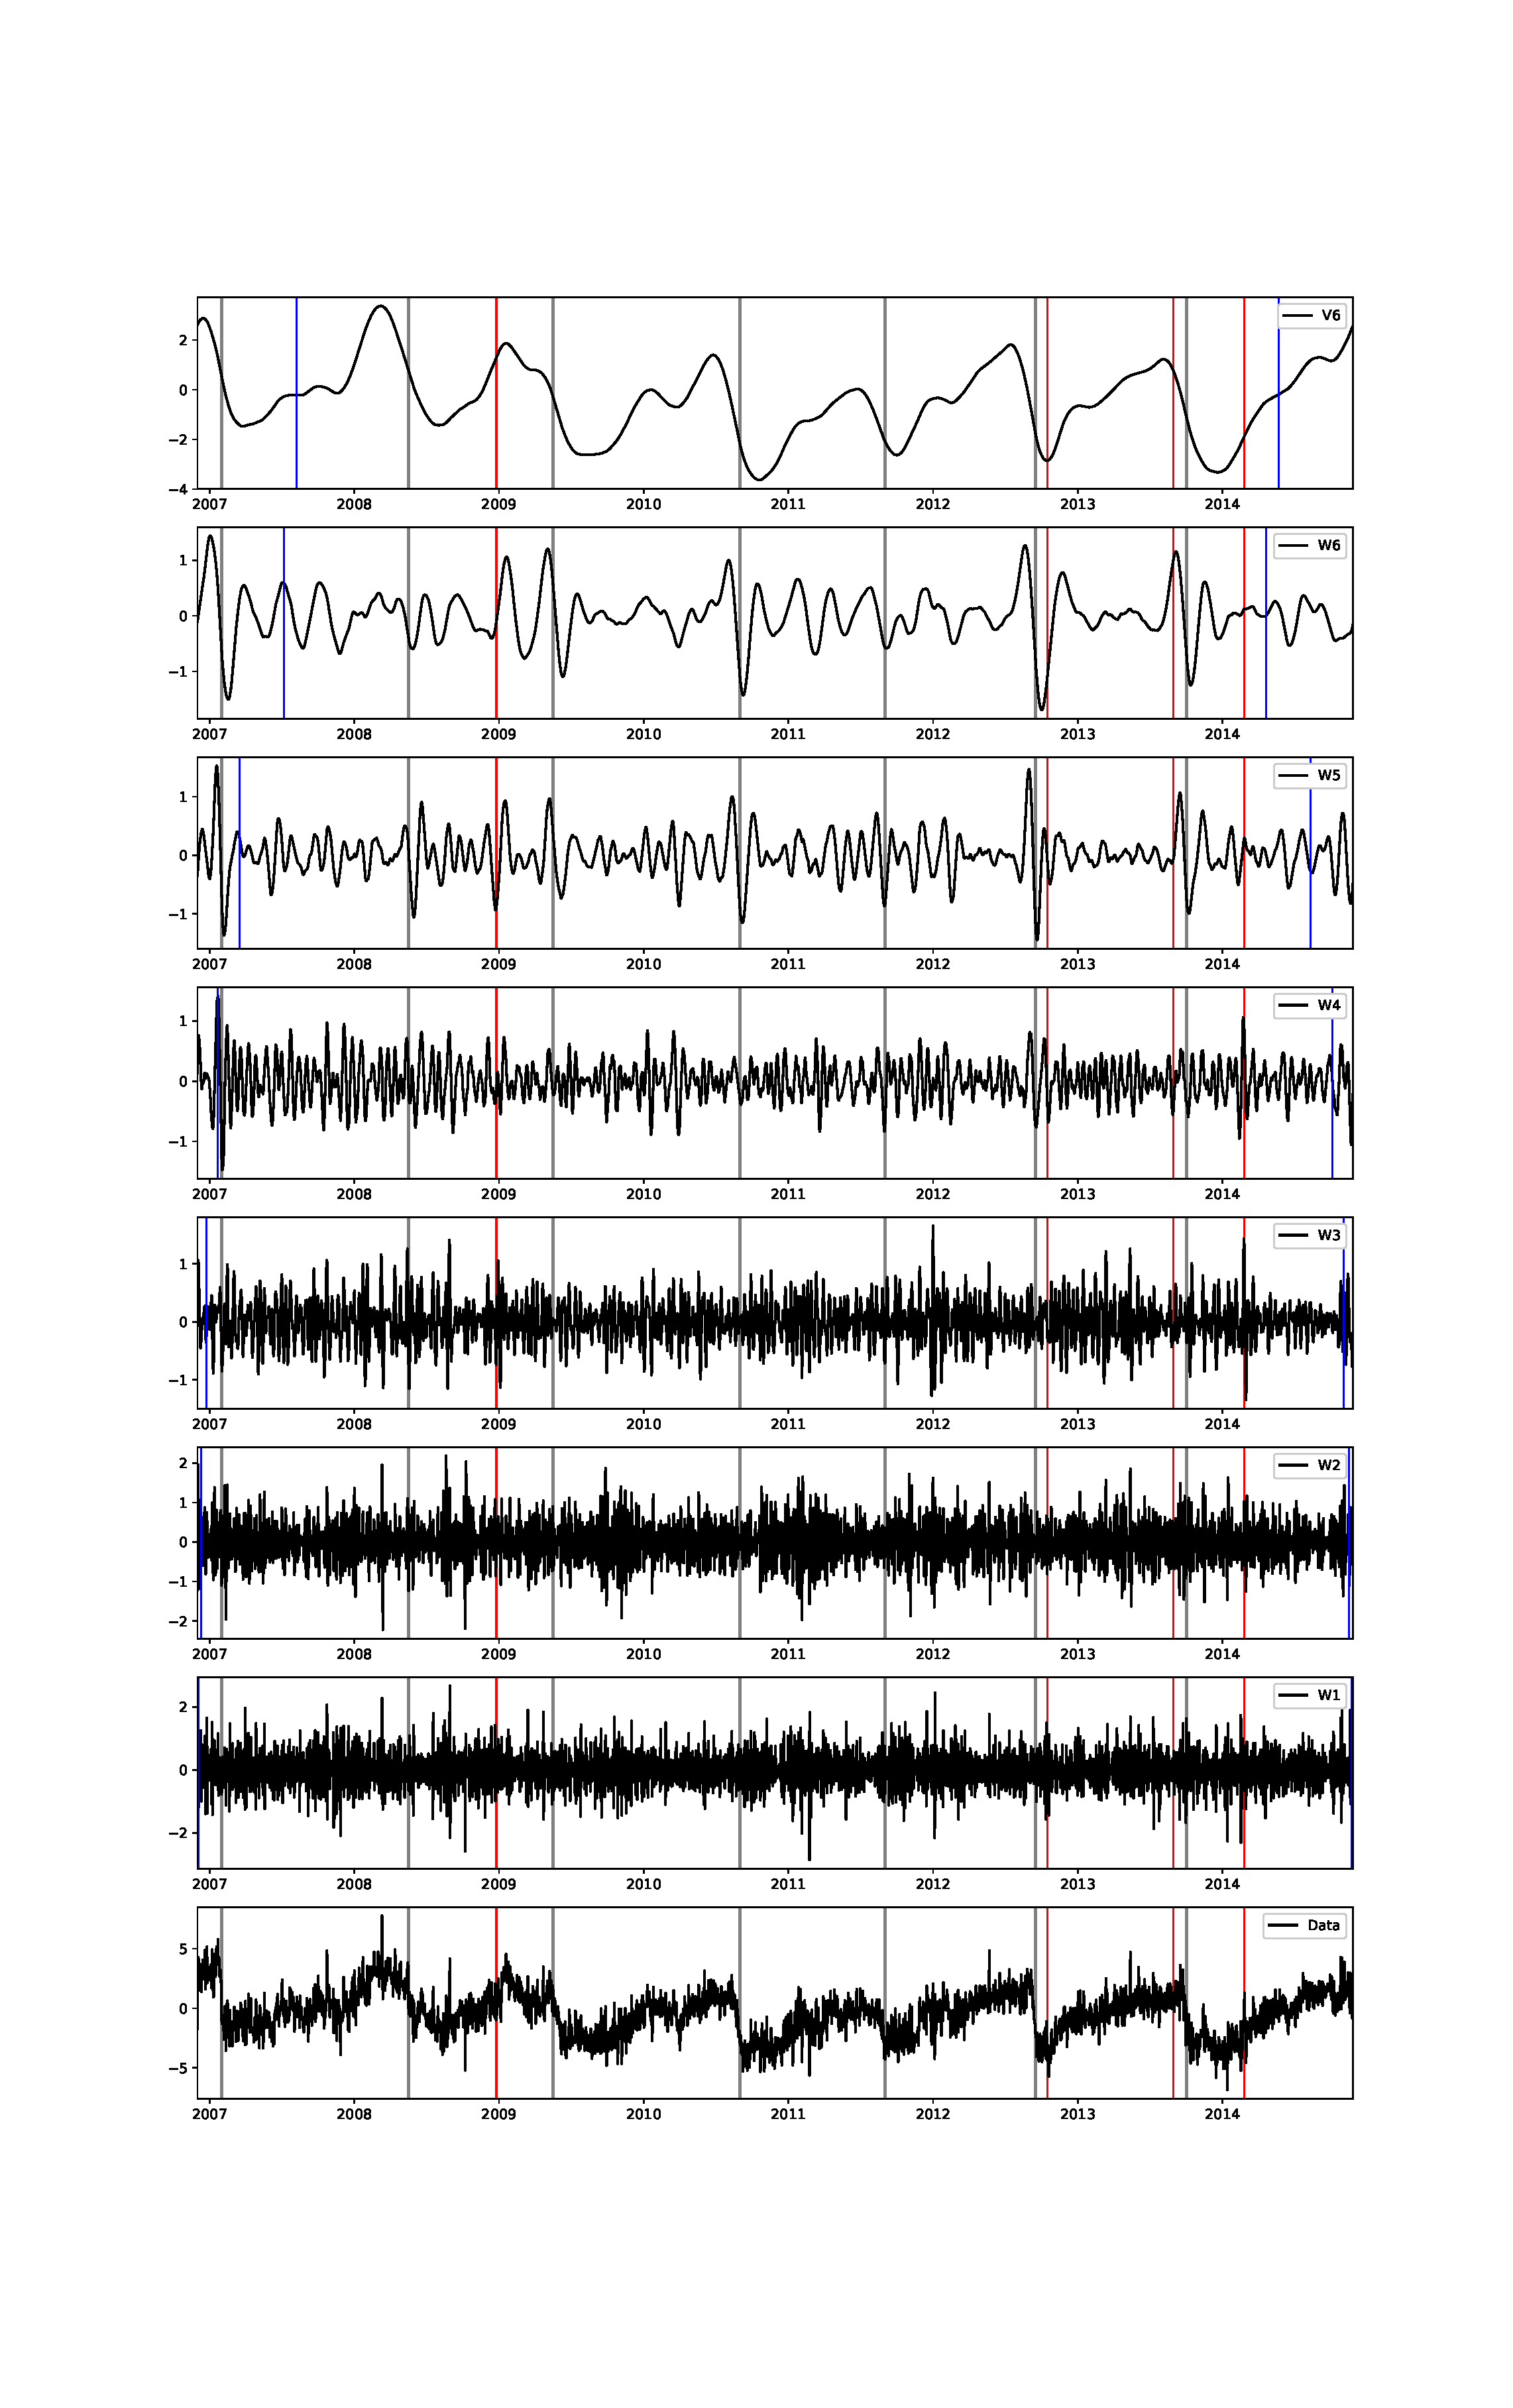
\includegraphics[width=300pt, trim={3.5cm 6cm 3.5cm 6.5cm},clip]{Figures/slowslip_results/Figure_3.eps}
\captionsetup{type=figure}
\captionof{figure}{Partial MODWT wavelet coefficients up to level 6 of the longitudinal component of station PGC5. The red bars correspond to the days where data were missing. The grey bars correspond to the timing of ETS events. The blue bars correspond to the left and right boundaries outside of which the wavelet coefficients are affected by the boundary conditions.}
\end{center}

Finally, the 5\textsuperscript{th} and 6\textsuperscript{th} level details of the MRA are plotted with the cumulative number of tremor in Figure 20.4. Peaks corresponding to the August 2010, September 2012 and September 2013 ETS events can clearly be seen in both the 5\textsuperscript{th} and the 6\textsuperscript{th} level details. Peaks that could corresponds to the August 2011 ETS event, and a small inter-ETS event in March 2010, can also be seen in the 5\textsuperscript{th} level detail, but this is less obvious than for the other ETS events.

\begin{center}
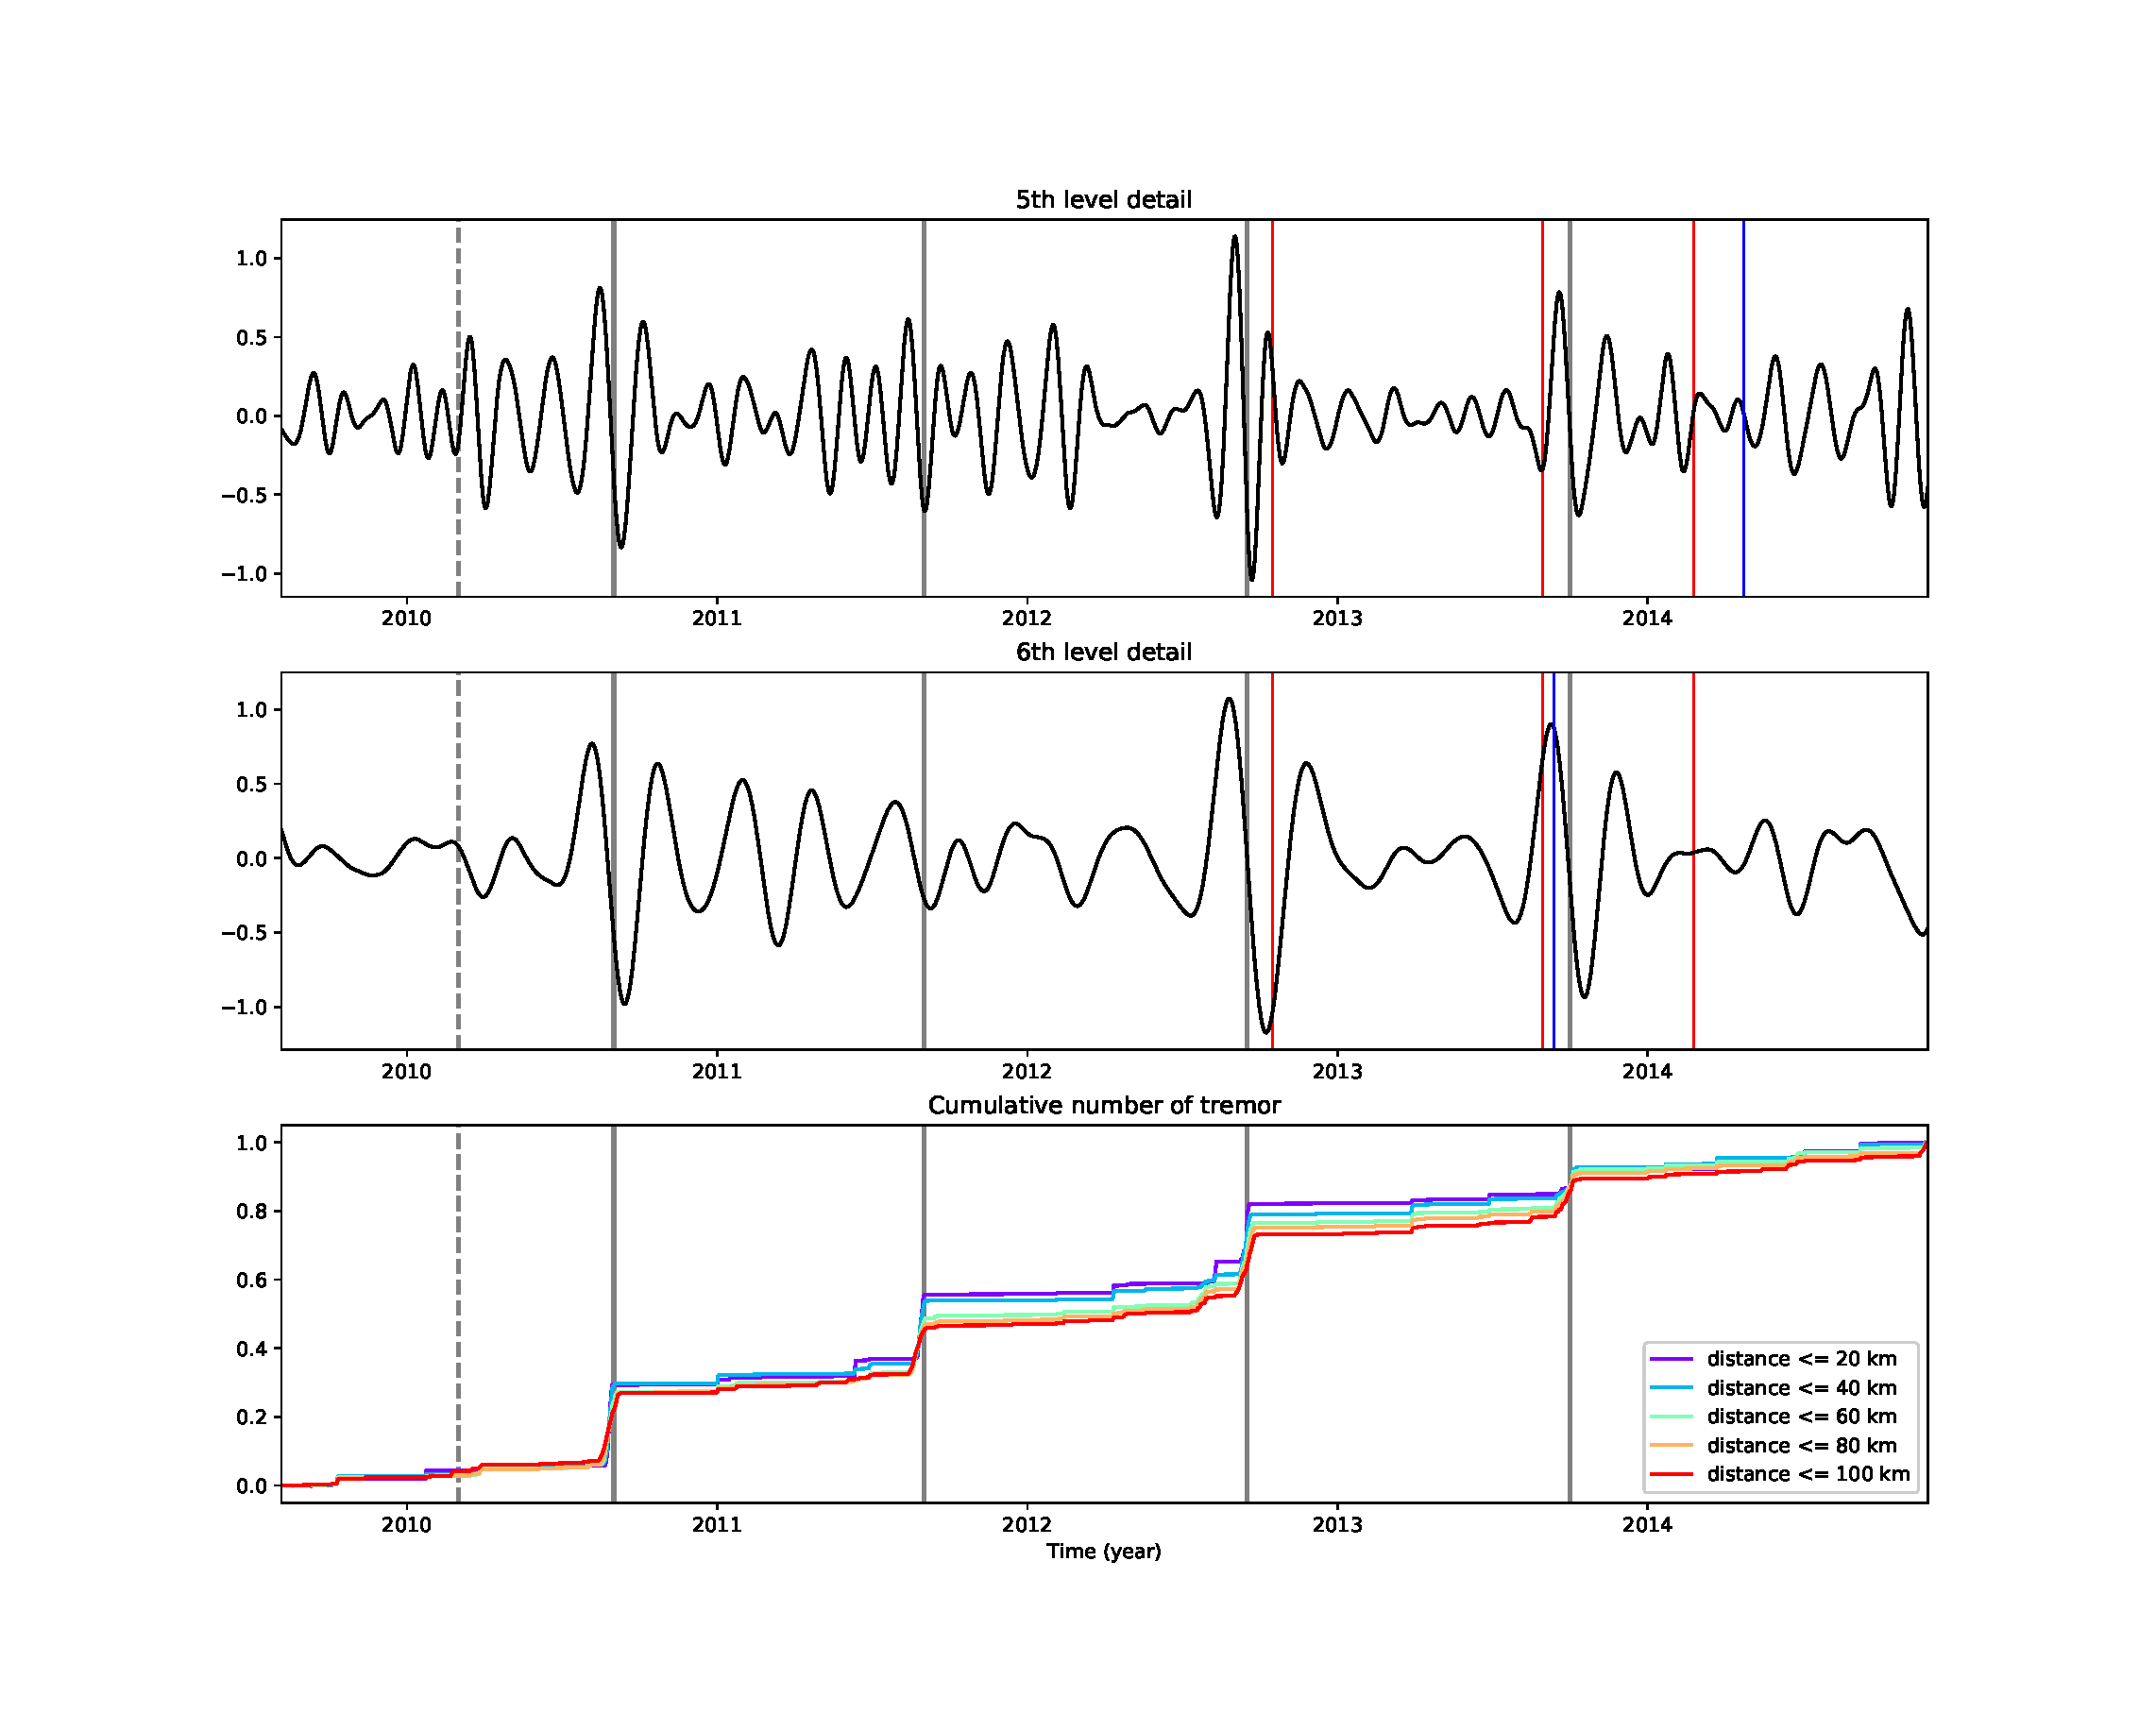
\includegraphics[width=300pt, trim={3.5cm 2.5cm 3.5cm 3cm}, clip]{Figures/slowslip_results/Figure_4.eps}
\captionsetup{type=figure}
\captionof{figure}{5\textsuperscript{th} and 6\textsuperscript{th} level details of the partial MODWT analysis of the longitudinal component of station PGC5 (top and middle panel), and cumulative number of tremor recorded around the GPS station (bottom panel). The red bars correspond to the days where data were missing. The grey bars correspond to the timing of ETS events. The blue bar corresponds to the right boundary outside of which the wavelet coefficients are affected by the boundary conditions.}
\end{center}

We did a similar analysis with the longitudinal component of the displacement at GPS stations CLRS, CUSH, FRID, PNCL, PTAA, and SQIM, all located in the Olympic Peninsula, or on Vancouver Island, and we found similar results. The 5\textsuperscript{th} and 6\textsuperscript{th} level details of the MRA for each of these stations is plotted as function of the latitude of the stations in Figures 20.5 and 20.6. For the 5\textsuperscript{th} level detail, we can see a peak corresponding to the August 2010 ETS event for stations FRID, PNCL, SQIM, and CUSH. The September 2012 ETS event can be seen for stations CLRS, PGC5, PTAA, and CUSH. The September 2013 ETS event can be seen for stations CLRS, PGC5, and PTAA. The January 2016 ETS event can be seen for stations CLRS, PGC5, FRID, PTAA, and CUSH. Finally, the March 2017 ETS event can be seen for stations CLRS, PGC5, and PTAA.

\begin{center}
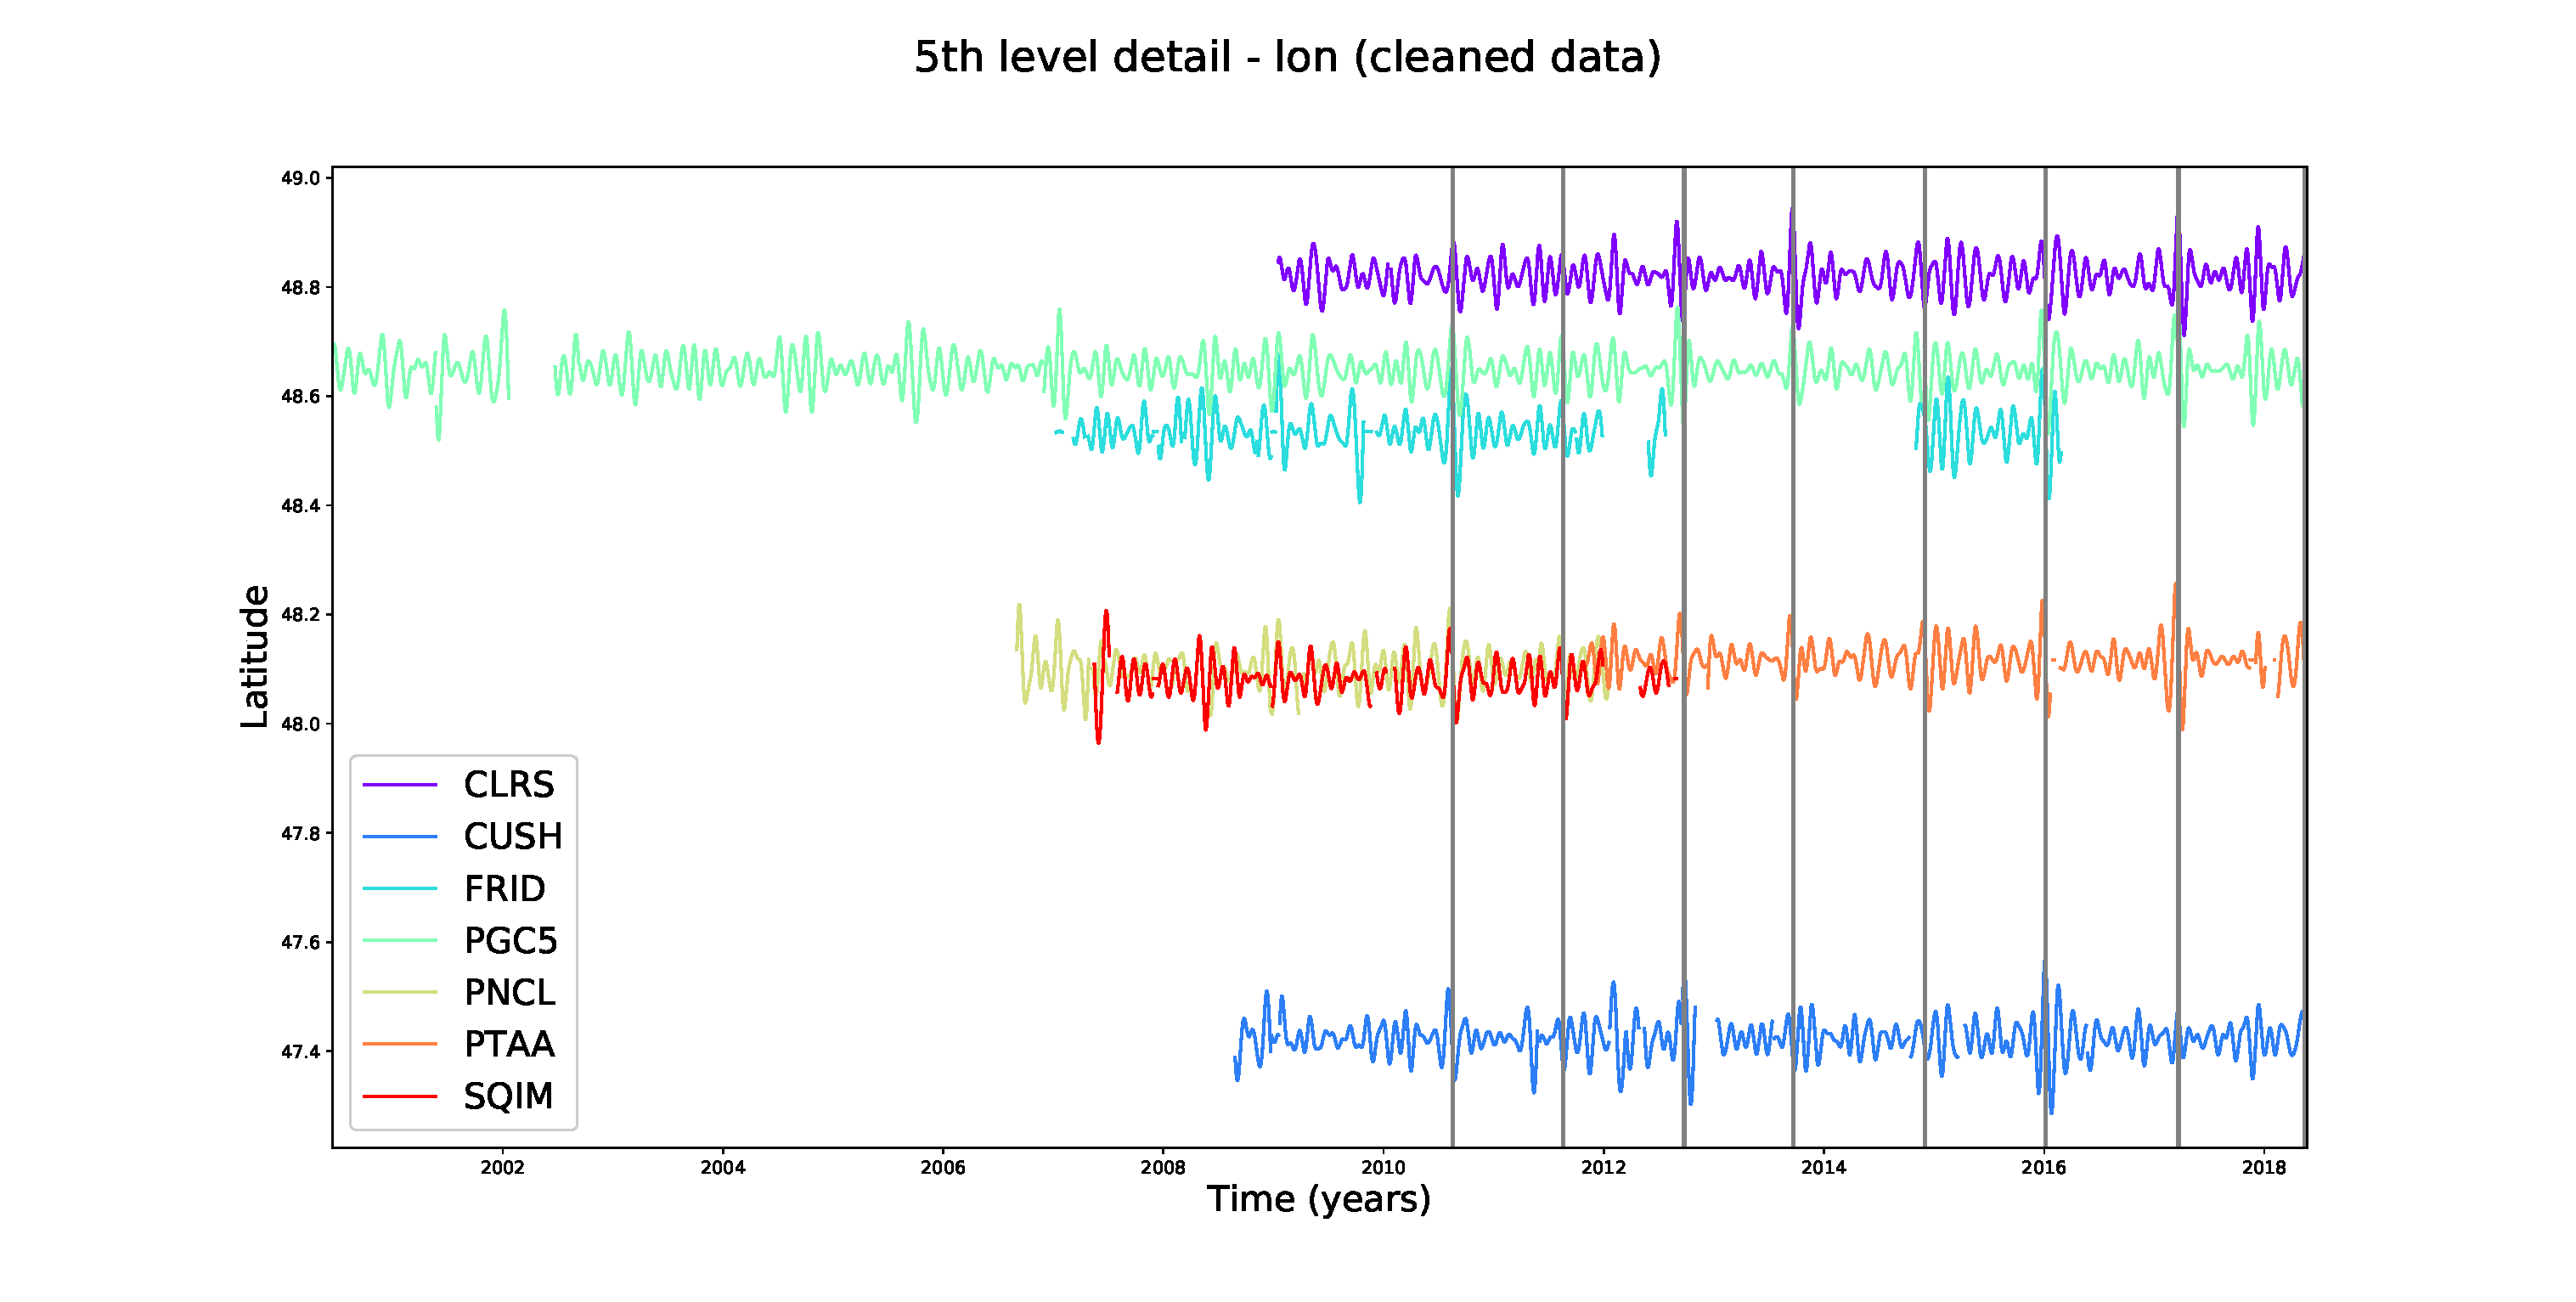
\includegraphics[width=500pt]{Figures/slowslip_results/Figure_5.eps}
\captionsetup{type=figure}
\captionof{figure}{5\textsuperscript{th} level detail of the partial MODWT analysis for GPS stations CLRS, CUSH, FRID, PGC5, PNCL, PTAA, and SQIM, as function of the latitude of the stations. The grey bars correspond to the timing of ETS events.}
\end{center}

For the 6\textsuperscript{th} level detail, we can see a peak corresponding to the August 2010 ETS event for stations PGC5, FRID, PNCL, and SQIM. The September 2012 ETS event can be seen for stations CLRS, PGC5, and PTAA. The September 2013 ETS event can be seen for stations CUSH, PGC5, and PTAA. The December 2014 ETS event can be seen for stations FRID, and PTAA. Finally, the January 2016 ETS event can be seen for stations PGC5, and FRID.

\begin{center}
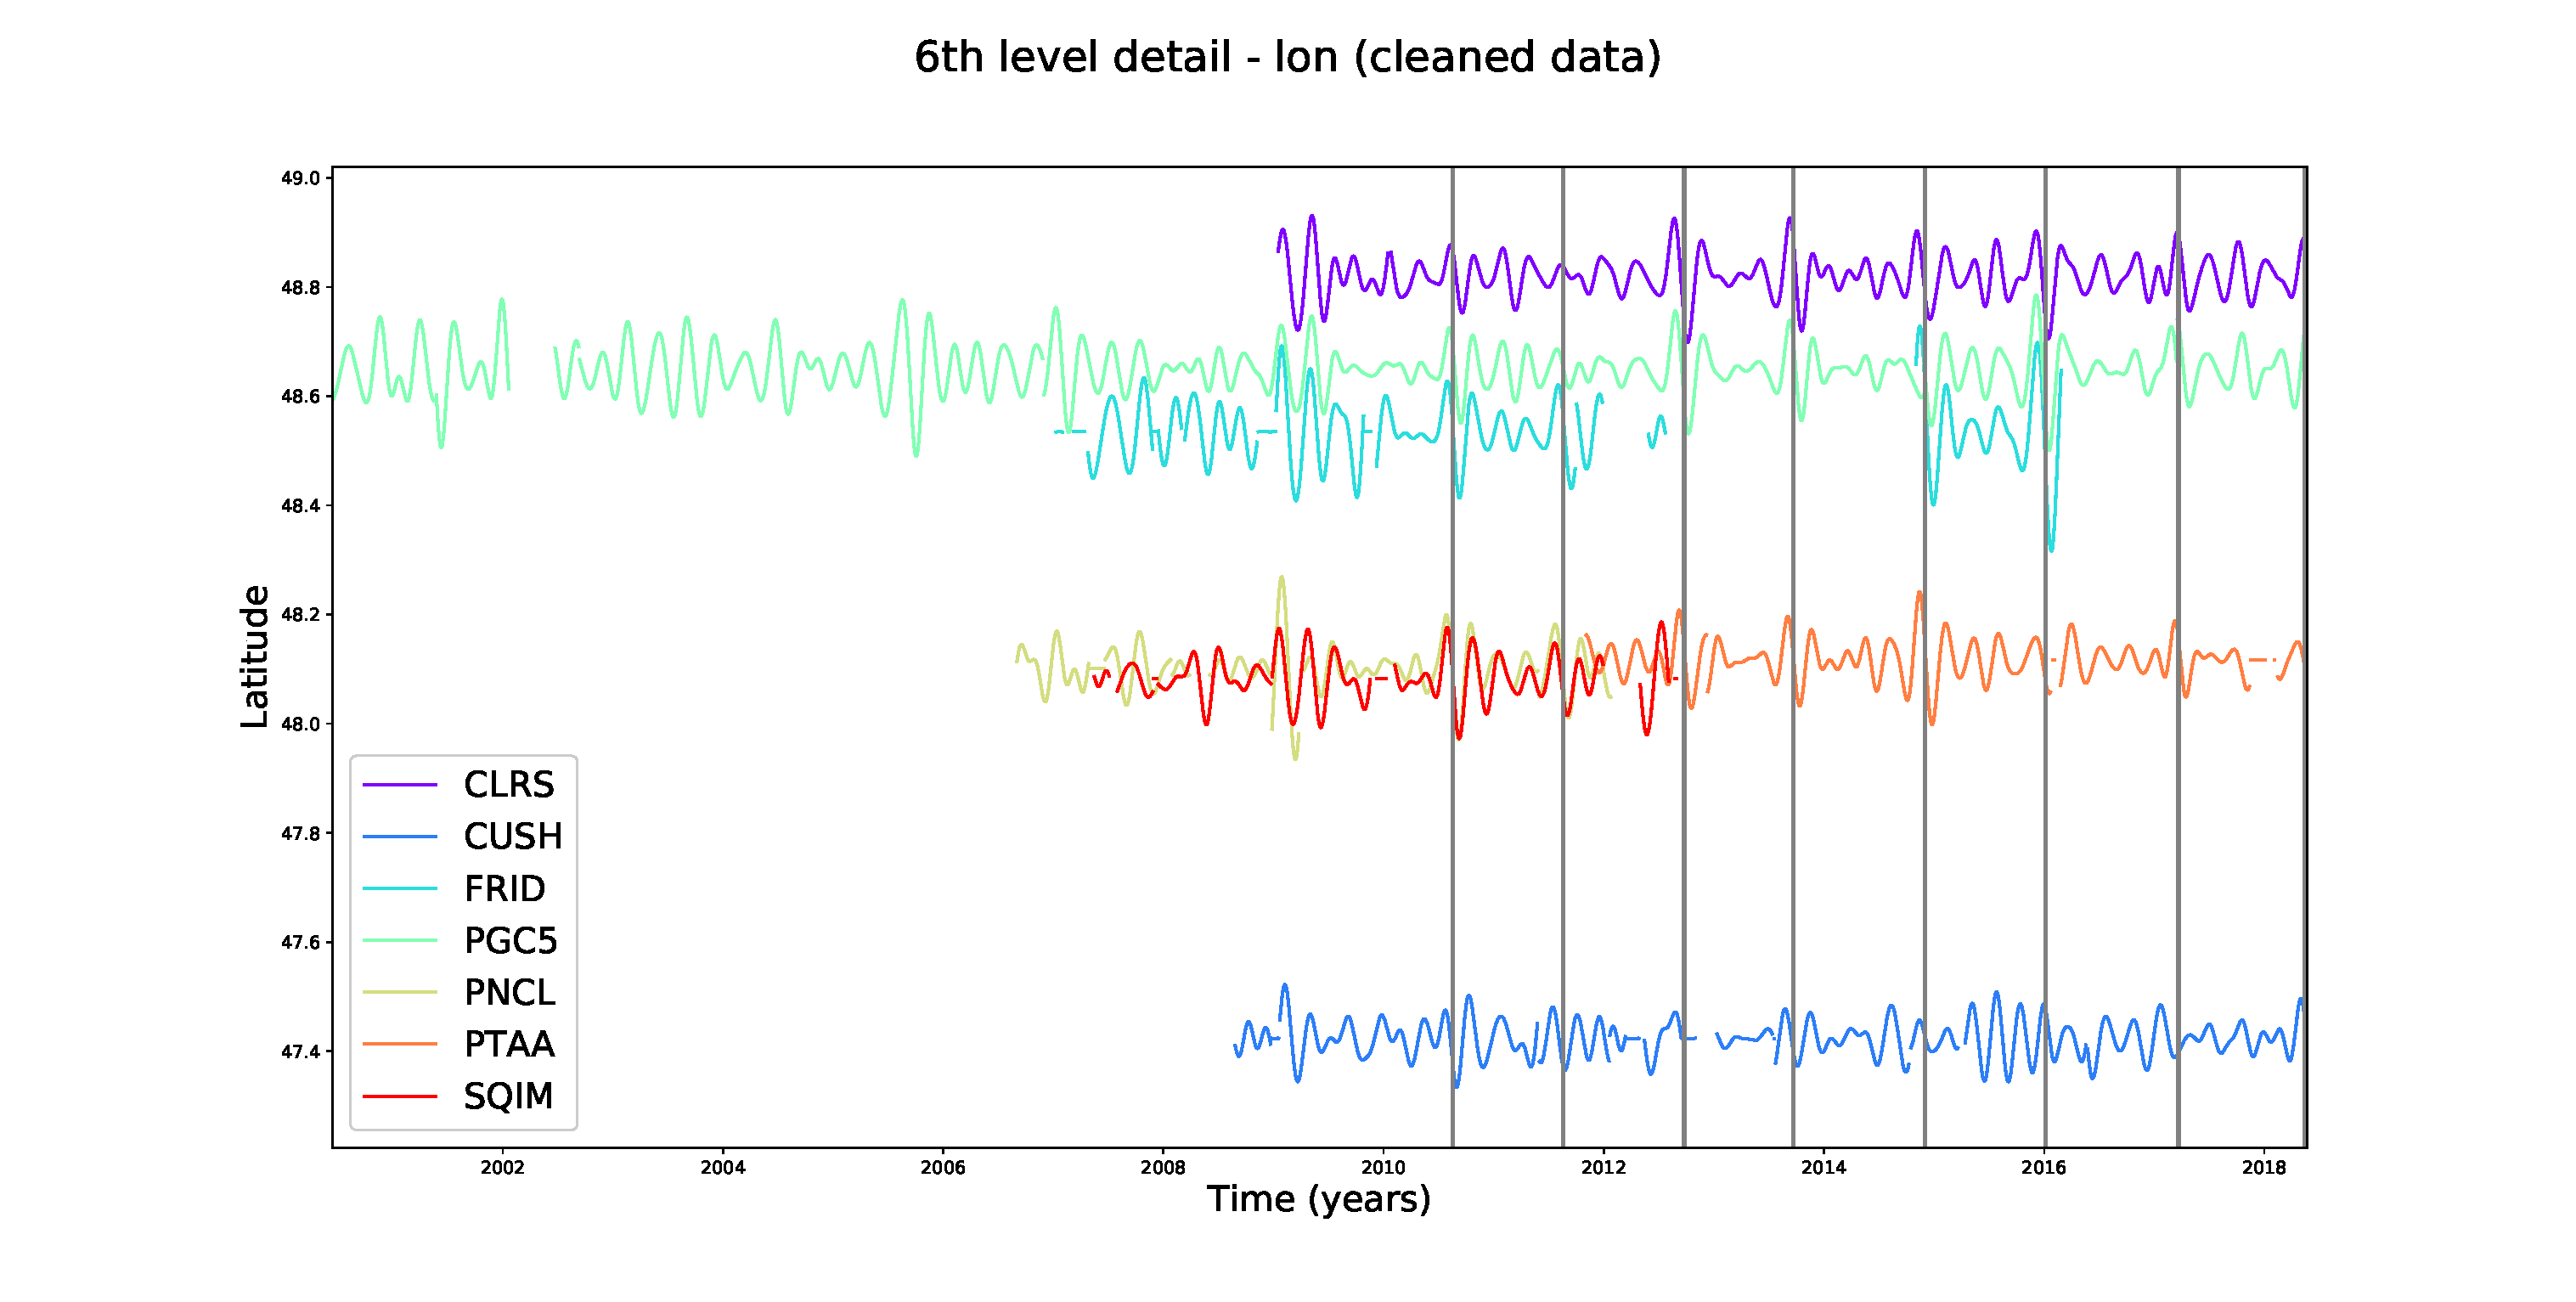
\includegraphics[width=500pt]{Figures/slowslip_results/Figure_6.eps}
\captionsetup{type=figure}
\captionof{figure}{6\textsuperscript{th} level detail of the partial MODWT analysis for GPS stations CLRS, CUSH, FRID, PGC5, PNCL, PTAA, and SQIM, as function of the latitude of the station. The grey bars correspond to the timing of ETS events.}
\end{center}

\chapter{Discussion and things to do}

Things to do:

\begin{itemize}

\item Change point detection: Can we detect a big ETS event starting, and when can we detect it? Before it becomes obvious due to the tremor recordings? We could test other wavelets (Daubechies with extremal phase may be a good idea), or look at the wavelet variance (see paper by Eric Moulines - Kouamo et al., 2011, with correction of the mistake in Percival's paper).

\item Plot of the cumulative number of tremor: How to get the exact timing of the inflection point / change point for putting it on the wavelet plot?

\item Implementation of matching pursuit: I hope to see among the first basis vectors the ones at level 5 and 6 that could correspond to the big ETS events, and maybe some others at level 4 that could correspond to smaller and shorter inter-ETS events.

\item Looking at what could do for the missing data points:
\begin{itemize}
	\item Linear or more complex interpolation
	\item Simply replace them with Gaussian noise
	\item Look at what we can do with kriging
\end{itemize}

\item Doing a test with a synthetics time series, and look at what we can see (level where we see the slow slip compared with duration, influence of an outlier, missing data, noise, inflence of different types of wavelets)

\item Test other wavelets with MODWT details

\item Regions to look at: New Zealand (slow slip but no tremor), Alaska (5 years long slow slip events)

\item For NASA fellowship, see Scott Henderson and glaciology students + speak about three points:
\begin{itemize}
	\item The science
	\item The societal aspect (natural hazards)
	\item The technique: the idea is to develop a method, exploit GPS data, pull out signals, make it more useful, maybe it could be applied to other types of phenomena
\end{itemize}

\end{itemize}

\section{Broader impacts}

Broader impacts = Answer to the following questions:
\begin{itemize}
\item Societal benefit, improve life on our planet, assess and respond to natural hazards and extreme events, inform decisions and provide benefits to society
\item Develop a method, exploit GPS data, pull out signals, make it more useful
\item Emphasis on the utilization of NASA's unique capabilities (fleet of Earth observing satellite)
\item Science + societal + techniques
\item Other types of phenomena that could be analyzed with the same methods
\end{itemize}

\subsection{Better understanding of the seismic hazard}

The largest earthquakes on Earth occur in subduction zones, where large segments of the plate boundary can store energy for centuries and then release it in minutes. A better understanding of subduction zone processes is thus necessary to study the associated seismic hazard. Moreover, slow slip and tremor events have a relatively short recurrence time, compared to the earthquake cycle that can last for hundreds of years, allowing scientists to observe and study complete event cycles, which are typically not possible to explore with traditional earthquake catalogs. Finally, slow slip occurs in a section of the plate boundary adjacent to the locked section of the subduction zone. This transient motion thus complicates our understanding of the earthquake cycle, as interactions between the slow slip zone and the seismogenic zone could potentially trigger large earthquakes, and should be taken into account when studying the seismic hazard. \\

Specifically, a better measurement of the vertical displacement at the Earth's surface during slow slip events is necessary to better constrain the depth extent of the slip area at the plate boundary. The up-dip limit of the slow slip area is assumed to constrain the down-dip limit of the megathrust earthquake rupture, a variable that is useful for seismic hazard studies, and the design of building codes. Constraining the down-dip limit of slow slip is also useful to estimate the area that slips during a slow-motion earthquake, and thus the percentage of the plate convergence that is released by large slow slip episodes. Additionally, the up-dip and down-dip limits of slow slip can be correlated with other geophysical data, such as porosity, temperature, and structure, in an effort to better understand the underlying processes that facilitate aseismic slip. \\

Moreover, being able to detect smaller, currently undetected slow slip events would help us to verify whether the fault weakens with depth. Indeed, it has been observed that, with increasing depth, there is a gradation from frequent tremor episodes with small spatial and temporal extent, to infrequent tremor episodes with large spatial and temporal extent. The same behavior was observed for low-frequency earthquakes (LFEs) with downdip LFE swarms happening nearly weekly and up-dip families only occurring during the yearly Episodic Tremor and Slip (ETS) events. As there is a temporal and spatial correlation between slow slip, tremor and LFEs, the same spatial pattern is also expected for the slow slip. However, the limited resolution of geodetic instruments only allows us to observe the largest slow slip events, and many smaller slow slip events may be undetected. It has been hypothesized that stable sliding at depth transfers stress to the base of the ETS zone, initiating frequent tremor and small slow slip. In a self-similar process, stress is then transferred up-dip of the fault, triggering less frequent tremor and larger slow slip, up toward the locked zone. This unobserved up-dip slip could help mediate plate convergence and either lower the slip deficit available for co-seismic slip or shift the downward extent of the megathrust rupture away from urban centers. \\

\subsection{Extension of the method to the study of other phenomena}

One of the main objectives of this research project is to develop a wavelet method to carry out analyses of GPS time series, and make GPS datasets more helpful for the study of physical phenomena. \\

Indeed, wavelet methods combined with GPS measurements have already been used for instance for monitoring bridge deformation. Kaloop and Li (2015 ~\cite{KAL_2011}) used the Discrete Wavelet Transform to detect abrupt changes in the GPS response by decomposing the signal into approximation and detail levels. Wavelet methods are also used for noise reduction of GPS observations, and improvement of the accuracy of the GPS time series (Kaloop and Kim, 2016 ~\cite{KAL_2016}). \\

It is important to monitor the displacement time series and to explore the failure mechanism of reservoir landslide for early warning. Traditionally, it is a challenge to monitor the landslide displacements real-timely and automatically. Globe Position System (GPS) is considered as the best real-time monitoring technology, however, the accuracies of the landslide displacements monitored by GPS are not assessed effectively. A web-based GPS system is developed to monitor the landslide displacements real-timely and automatically in this study. And the discrete wavelet transform (DWT) is proposed to assess the accuracy of the GPS monitoring displacements. In this study, the wavelet analysis (WA) is proposed to assess the accuracy of the GPS monitoring landslide displacements
A web-based GPS system for displacement monitoring and failure mechanism analysis of reservoir landslide
Li, Yuanyao ; Huang, Jinsong ; Jiang, Shui-Hua ; Huang, Faming ; Chang, Zhilu
Sci Rep, 2017, Vol.7(1), pp.17171-17171 \\



develop  a  robust  GPS  signal acquisition  system  that  improves  the  performance  of  the  system  over  noisy  transmission  channel and  in  the  presence  of  other  sources  of  noise.  An  acquisition
  algorithm  based  on  DWT is  proposed  for  a  robust GPS  signal acquisition  system  and  to  facilitate  its  implementation.
Acquisition is the first signal processing operation performed on the IF GPS signal. Acquisition identifies the satellites visible to the receiver and provides the estimation of the Doppler shift in carrier frequency and delay
in C/A code of the satellite signals. These parameters  are  given  as  input  to  the  tracking,  is  used  to  find  the  phase  transition  of  the  navigation  data.  After  identifying the available satellites and acquiring their signal parameters, tracking is done through parallel channels. In tracking, C/A code and carrier are removed by measurement of the code phase and Doppler frequency precisely. So  performance  of  acquisition  processes  directly influence  the  performance  of  tracking  operation.  The  most  affecting source  of  acquisition  error  is  due  to  the  noise  on  the  transmission  channel.  The  presenceof  the  noise  affects seriously the precision in the measurements of acquisition process. 
A Robust GPS Signal Acquisition Technique Using Discrete Wavelet Transform
Ahamed, Shaik Fayaz ; Rao, G. Sasibhushana ; Ganesh, L.
Procedia Computer Science, 2016, Vol.85, pp.683-690 \\

Repeatable satellite orbits can be used for multipath mitigation in GPS-based deformation monitoring and other high-precision GPS applications that involve continuous observation with static antennas. Multipath signals at a static station repeat when the GPS constellation repeats given the same site environment. Repeat-time multipath filtering techniques need noise reduction methods to remove the white noise in carrier phase measurement residuals in order to retrieve the carrier phase multipath corrections for the next day. We propose a generic and robust three-level wavelet packets based denoising method for repeat-time-based carrier phase multipath filtering in relative positioning; the method does not need tuning to work with different data sets.

Wavelet packets based denoising method for measurement domain repeat-time multipath filtering in GPS static high-precision positioning
Lau, Lawrence
GPS Solutions, 2017, Vol.21(2), pp.461-474 \\

Multipath remains one of the major challenges in Global Navigation Satellite System (GNSS) positioning because it is considered the dominant source of ranging errors. Urban situations in particular are affected by this phenomenon, yielding several blunders in the measurements and unacceptable errors in the navigation solution. Multipath is caused by multiple signal reflections from various objects in the environment; multipath signals are always delayed compared to line-of-sight signals.
Multipath remains one of the major challenges in Global Navigation Satellite System (GNSS) positioning because it is considered the dominant source of ranging errors, which can be classified into specular and diffuse types. We present a new method using wavelets to extract the pseudorange multipath in the time domain and breaking it down into the two components. The main idea is an analysis-reconstruction approach based on application of both continuous wavelet transform (CWT) and discrete wavelet transform (DWT).
A new method for specular and diffuse pseudorange multipath error extraction using wavelet analysis
Pugliano, Giovanni ; Robustelli, Umberto ; Rossi, Fabio ; Santamaria, Raffaele
GPS Solutions, 2016, Vol.20(3), pp.499-508 \\


GPS uses a direct sequence spread-spectrum (DSSS) signal that is highly susceptible to interference, which may be both intentional and nonintentional. The primary area of concern in both commercial and military applications is the protection from intentional interferers. Development of techniques for the protection of GPS from interference and jamming is an area of active research.
Hence, a discrete wavelet transform (DWT) filter using a biorthogonal wavelet is suggested and its performance analyzed here for single and multiple FM (frequency modulation) interference suppression.
New approach for suppression of FM jamming in GPS receivers
Deergha Rao, K. ; Swamy, M.N.S.
IEEE Transactions on Aerospace and Electronic Systems, October 2006, Vol.42(4)

\subsection{Data management}

All scripts used to carry out the wavelet analysis and generate the figures are written with Python, and are available on the student's GitHub repository. Jupyter notebooks explaining in a more detailed manner the wavelet analysis are also available on GitHub. All future scripts developed during this research project will be made available to the public in a similar way.

\end{document}
